\chapter{Methodology} \label{ch:methodology}

In this chapter, our \acrshort{wsol} evaluation methodology is explained in detail. We specify the different networks and datasets used to train models and evaluate localization methods. Then, we explain how training of the models is done. The localization in general and specifically for each localization method is discussed in detail. Finally we define how we aim to improve localization of multiple-instances for the \acrshort{wsol} task.

\section{Networks}
The \acrshort{cam}-based \acrshort{wsol} methods require a \acrshort{cnn} model to classify images and localize objects in those images. We use the VGG16 and ResNet-50 network. The VGG16 and a variant with \acrshort{gap} layer, are used in a many papers \cite{zhou2016cvpr, selvaraju2017grad, chattopadhyay2017grad, wang2020score, wang2021minmaxcam} of the \acrshort{cam} family of methods. It is therefore a good reference for benchmarking \acrshort{wsol}. ResNet-50 is more recent than VGG16 and is used for experiments with MinMaxCAM by Wang, Kaili \textit{et al.} \cite{wang2021minmaxcam}.

\subsection{VGG16}
VGG16 is a \acrshort{cnn} proposed by K. Simonyan \textit{et al.} \cite{simonyan2014very}. It is one of the most popular models for image classification and it achieves high test accuracy for ImageNet, which is a very large dataset with 1000 different classes.
\begin{figure}[ht]
    \begin{center}       
    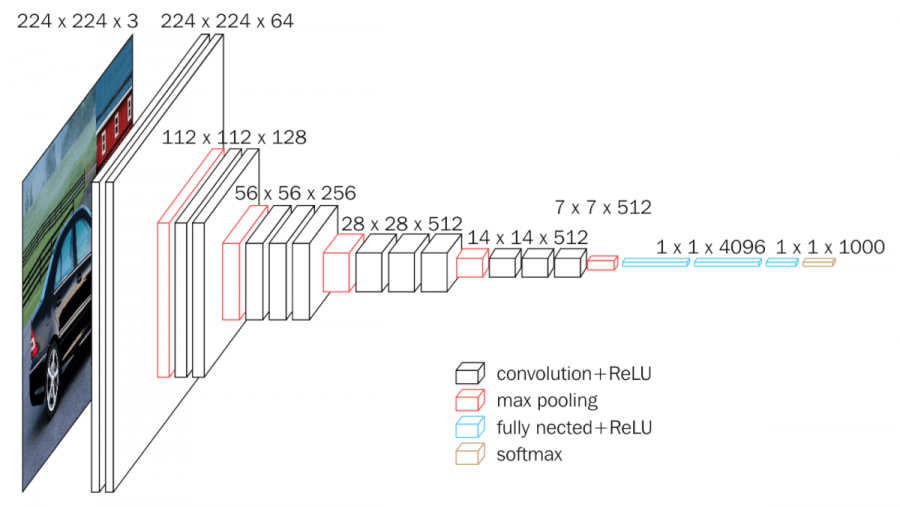
\includegraphics[width=1.0\textwidth]{fig_vgg16_arch.png}
    \caption[VGG16 architecture]{VGG16 architecture.}
    \caption*{Source: \href{https://neurohive.io/en/popular-networks/vgg16}{https://neurohive.io/en/popular-networks/vgg16}}
    \label{fig:vgg16_arch}
    \end{center}
\end{figure}

The VGG16 network architecture is shown in Fig. \ref{fig:vgg16_arch}. The 16 in VGG16 refers to 16 layers that have trainable weights. In VGG16 there are thirteen convolutional layers, five maximum pooling layers, and three dense layers. In Fig. \ref{fig:vgg16_arch}, each layer in the network is tagged with the dimensions of its output in a color that represents its function. Fig. \ref{fig:vgg16_layers_auth} tags the network layers with unique names that we will use to refer to those layers. Convolutional layers are organized in a number of sequences of layers. Layers within a sequence have the same number of filters.
\begin{figure}[ht]
    \begin{center}       
    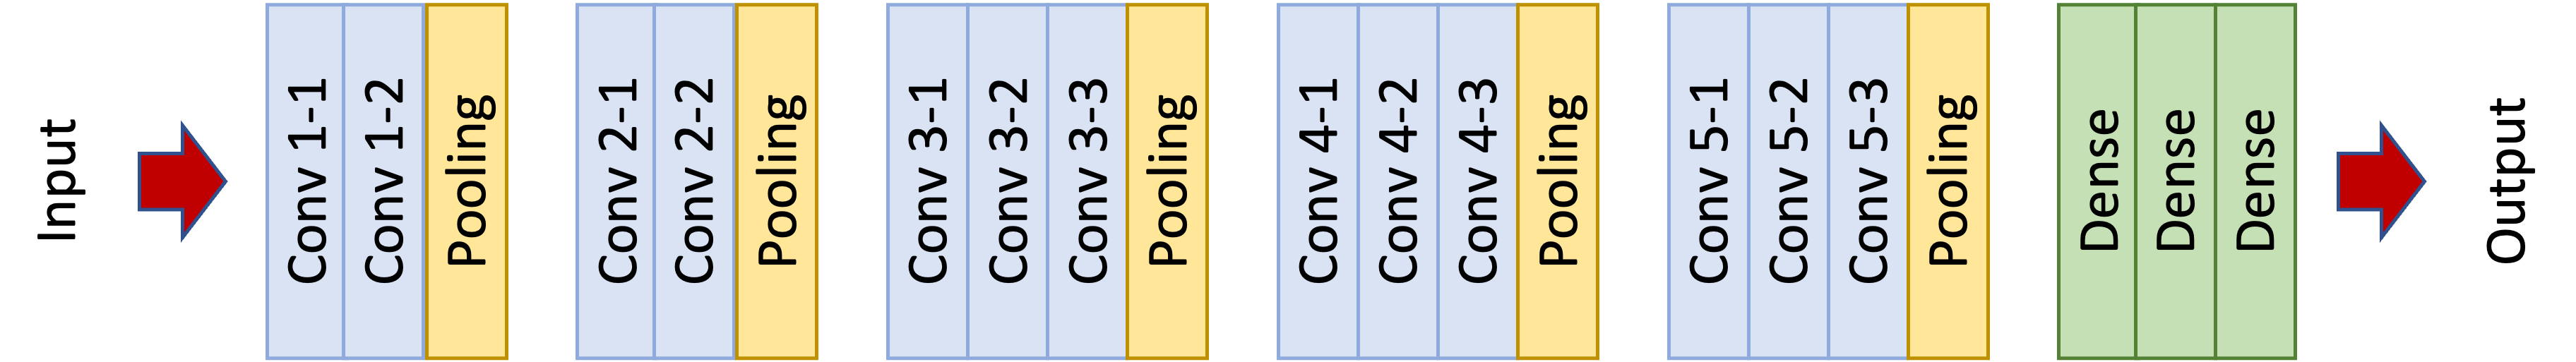
\includegraphics[width=1.0\textwidth]{fig_vgg16_layers_auth.png}
    \caption[VGG16 network layers]{VGG16 network layers.}
    \caption*{Source: Author}
    \label{fig:vgg16_layers_auth}
    \end{center}
\end{figure}

In subsequent sections, we describe the different parts of the architecture.
\subsubsection{Input}
The model expects as input images of fixed size and color channels. The dimensions are 224$\times$224$\times$3, standing for width$\times$height$\times$color channels. Typically images in popular datasets (e.g., ImageNet) have different sizes, requiring transformation of the images to resize them to the expected input shape.

\subsubsection{Convolutional layers}
The convolutional layers use a small kernel size of 3$\times$3 in all layers, which enables the network to go deeper \cite{simonyan2014very}. Conv-1 has 2 layers with 64 filters, Conv-2 has 2 layers with 128 filters, Conv-3 has 3 layers with 256 filters, Conv-4 and Conv-5 each have 3 layers with 512 filters. The number of filters represents the output channels of each layer.

\subsubsection{Activation function}
Each convolutional layer is followed by a \acrfull{relu} component. This activation function is a non-linear function that provides a matching output for positive inputs and outputs zero for negative inputs. Deep \acrshort{cnn}s with \acrshort{relu}s learn faster than equivalent activation functions with saturating neurons as indicated by Krizhevsky \textit{et al.} \cite{krizhevsky2017imagenet}.

\subsubsection{Pooling layers}
A pooling layer follows a sequence of convolutional layers with the same kernel size. Pooling helps to reduce the size of the feature maps created by each convolution step. When the number of filters doubles, also the number of feature maps doubles. A pooling window of 2$\times$2 reduces the size of feature maps by four, keeping computational complexity balanced as we go deeper in the network.

\subsubsection{Fully connected layers}
Three \acrfull{fc} layers follow a stack of convolutional layers: The first two have 4096 channels each, the third performs 1000-way  classification and thus contains 1000 units (one for each class). The final layer is the soft-max layer. This layer ensures that the output values are transformed into confidence scores: Each output value is between 0 and 1 and the total sum of all outputs is 1.

Due to its depth and number of fully-connected nodes, VGG16 has 138 million weights with a storage size over 533MB. This puts high computational and storage requirements on training and storing a VGG16 model.

\subsection{VGG16-GAP}
Zhou \textit{et al.} \cite{zhou2016cvpr} found that convolutional units are able to localize objects despite being trained on image-level labels. Despite this fact, this ability is lost when fully-connected layers are used for classification. The authors concluded that by adding a \acrfull{gap} layer and modifying the dense layers, the localization ability of a \acrshort{cnn} can be kept until the final convolutional layer. We refer to this tweaked version of a VGG16 network as the VGG16-GAP network.

Zhou \textit{et al.} specified that the localization ability of the network improved when the last convolutional layer before \acrshort{gap} has a higher spatial resolution. Therefore VGG16 is tweaked as illustrated in Fig. \ref{fig:vgg16_gap_layers_auth}. The pooling layer and \acrshort{fc} layers after Conv-5 are removed, resulting in a feature map with resolution 14$\times$14. Then a convolutional layer Conv6-1 is added with kernel size 3$\times$3 and 1024 units, followed by a GAP layer and a \acrshort{fc} and softmax layer.
\begin{figure}[ht]
    \begin{center}       
    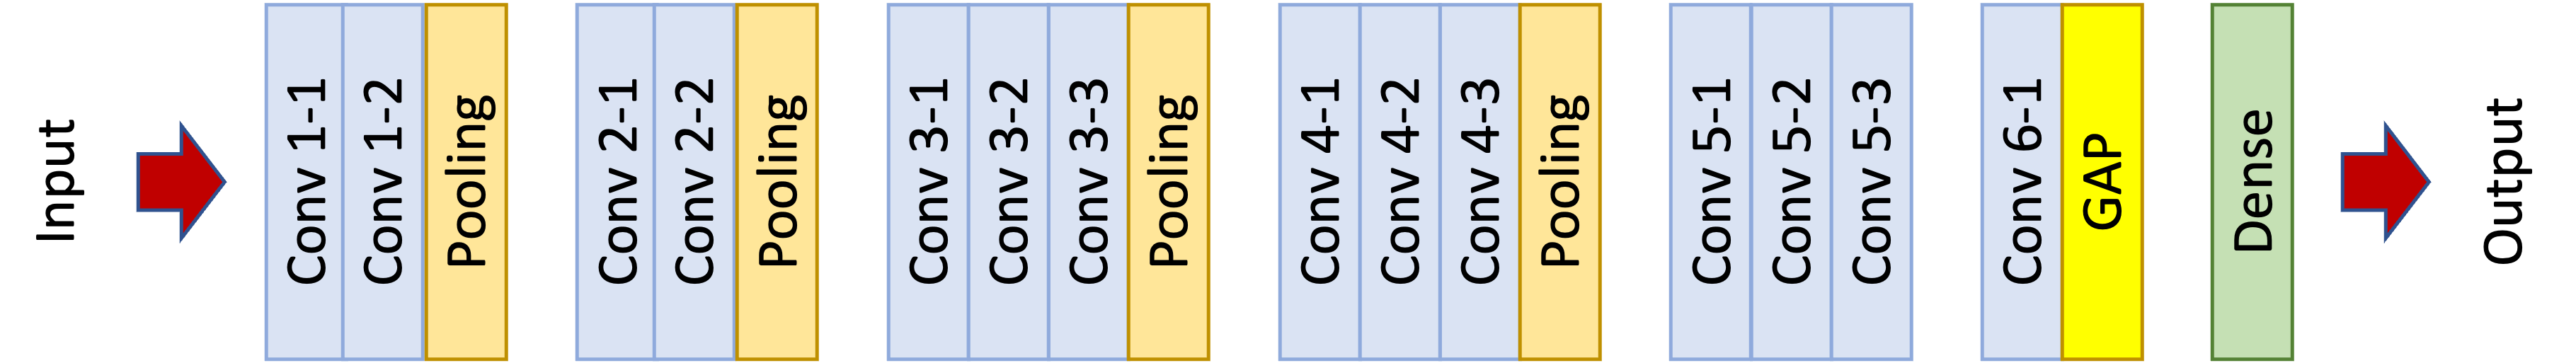
\includegraphics[width=1.0\textwidth]{fig_vgg16_gap_layers_auth.png}
    \caption[VGG16-GAP network layers]{VGG16-GAP network layers.}
    \caption*{Source: Author}
    \label{fig:vgg16_gap_layers_auth}
    \end{center}
\end{figure}

Note that removing fully-connected layers largely decreases the number of trainable network parameters: The VGG16-GAP network has 20 million parameters. The decrease in parameters also brings a classification performance drop. Zhou \textit{et al.} noticed an increase of 2\% points of the classification error on the ImageNet validation set, when modifying a VGG16 architecture to a VGG16-GAP architecture. 

\subsection{ResNet-50 network}
Network depth is of crucial importance in neural network architectures. The residual learning framework eases the training of these networks and enables them to be substantially deeper, leading to improved performance in both visual and non-visual tasks. These residual networks are much deeper than their ‘plain’ counterparts, yet they require a similar number of parameters (weights).

VGG16 introduced the concept of increasing the number of layers to improve accuracy. However, deeper networks are more difficult to train. He \textit{et al.} \cite{he2016deep} states that with network depth increasing, accuracy gets saturated and then degrades rapidly. This degradation leads to higher training error. The authors propose a solution to a deeper network that by construction should not have a higher training error than more shallow networks: The layers are copied from a learned shallower model and added layers are an identity mapping. The basic building block of residual networks is shown in Fig. \ref{fig:resnet_block}. The original non-residual mapping is cast into a residual mapping that should be easier to optimize. This basic building block is used in residual networks with 18 or 34 trainable layers. 
\begin{figure}[ht]
    \begin{center}       
    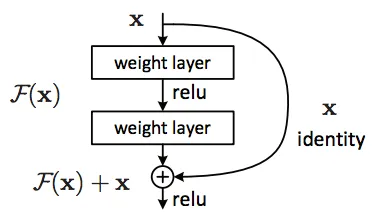
\includegraphics[width=0.4\textwidth]{fig_resnet_block.png}
    \caption[Residual block]{A residual. The fundamental building block of residual networks.}
    \caption*{Source: \href{https://medium.com/@waya.ai/deep-residual-learning-9610bb62c355}{https://medium.com/@waya.ai/deep-residual-learning-9610bb62c355}}
    \label{fig:resnet_block}
    \end{center}
\end{figure}

For deeper residual networks there is a concern on training time. Therefore, the basic building block is modified using a bottleneck design. An example is shown in Fig. \ref{fig:resnet_bottleneck}. For each residual function, a stack of three layers is used instead of two. The three layers are 1$\times$1, 3$\times$3, and 1$\times$1 convolutions, where the 1$\times$1 layers are responsible for reducing and then increasing dimensions, leaving the 3$\times$3 layer a bottleneck with smaller input/output dimension. For ResNet-50, all basic building blocks from ResNet-34 are replaced with bottleneck blocks, yielding 50 layers with learnable weights.
\begin{figure}[ht]
    \begin{center}       
    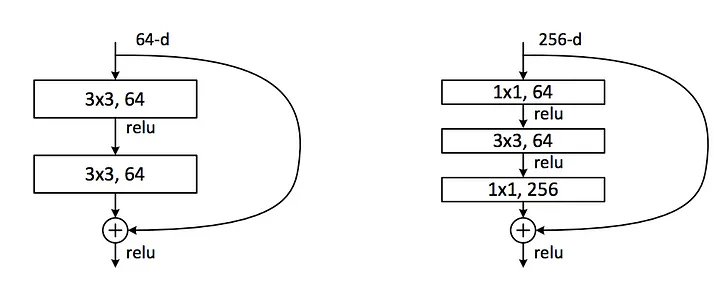
\includegraphics[width=0.7\textwidth]{fig_resnet_bottleneck.png}
    \caption[Residual basic and bottleneck blocks]{Basic residual block (left) and bottleneck residual block (right). Both designs have similar time complexity.}
    \caption*{Source: \href{https://medium.com/@waya.ai/deep-residual-learning-9610bb62c355}{https://medium.com/@waya.ai/deep-residual-learning-9610bb62c355}}
    \label{fig:resnet_bottleneck}
    \end{center}
\end{figure}

The detailed architecture of ResNet-50 and other variants are shown in Fig. \ref{fig:resnet_arch_table}. Although ResNet-50 has many more layers than VGG16, it has 25 million parameters which is far less than VGG16. 
\begin{figure}[ht]
    \begin{center}       
    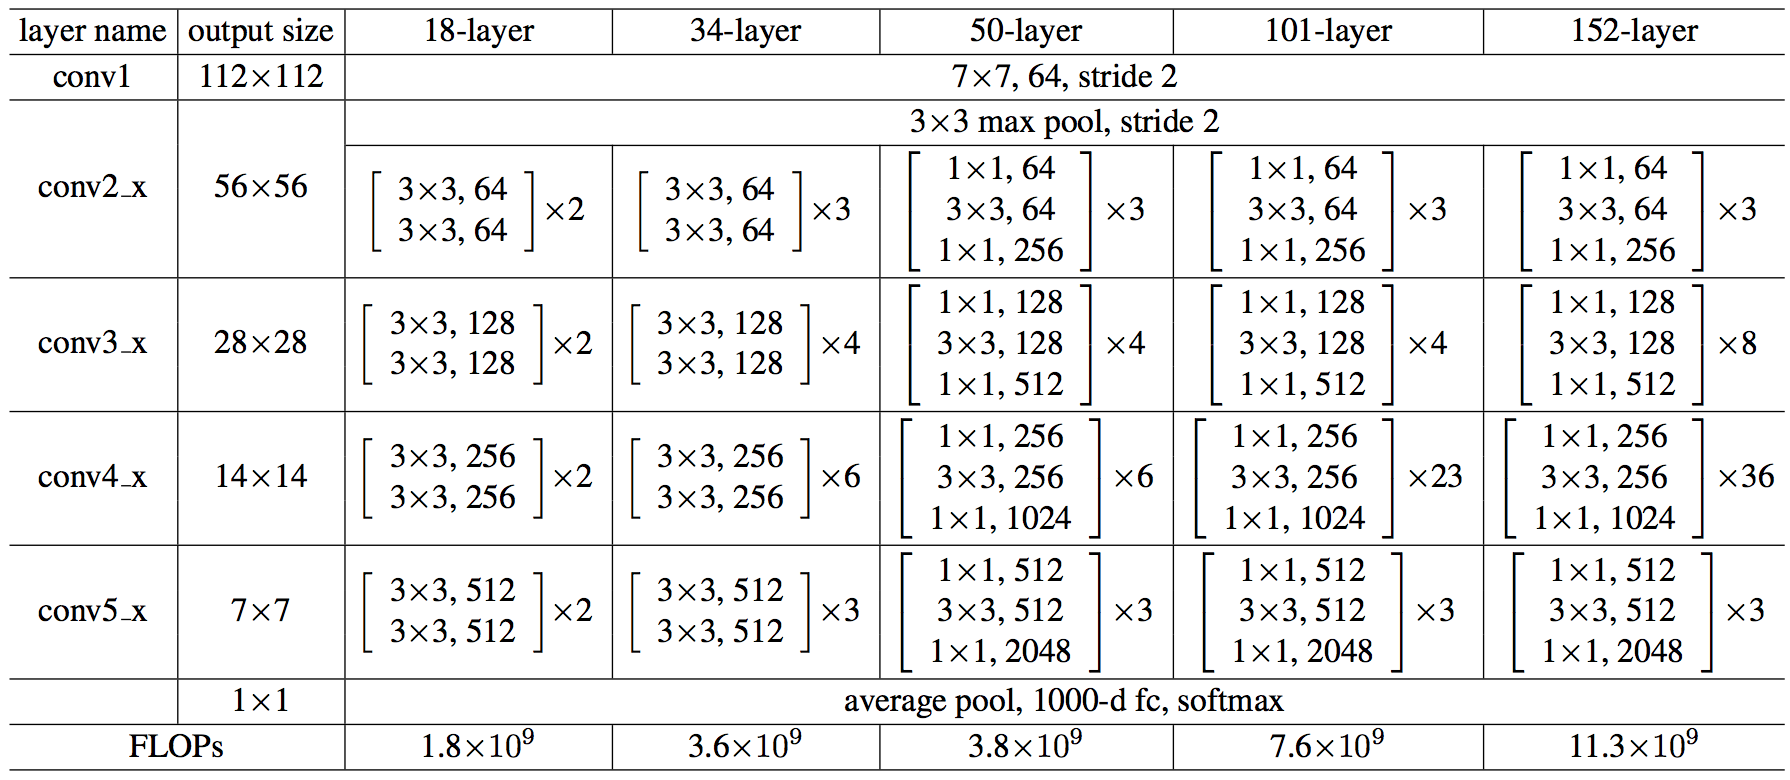
\includegraphics[width=1.0\textwidth]{fig_resnet_arch_table.png}
    \caption[Residual network architectures]{Residual network architectures for ImageNet. Building blocks are shown in brackets with the numbers of blocks stacked.}
    \caption*{Source: \href{https://neurohive.io/en/popular-networks/resnet}{https://neurohive.io/en/popular-networks/resnet}}
    \label{fig:resnet_arch_table}
    \end{center}
\end{figure}

\section{Datasets}
As most research papers evaluating \acrshort{cam}-related \acrshort{wsol} methods use the ImageNet dataset, we will use this dataset as well. Because ImageNet is a vast dataset and the our models (VGG16 and ResNet-50) are computationally demanding to train, we will also use a smaller synthetic dataset. This allows us to more quickly evaluate our assumptions and implementations.

\subsection{Synthetic dataset}
By using a synthetic dataset we limit computational requirements for training and evaluating our models. As we are evaluating localization of multiple object instances, using this synthetic dataset we have control over image structure, number of object instances and ground truth data. 

\subsubsection{Baseline}
For generation of the images, we took inspiration from Tjoa, E. \textit{et al.} \cite{tjoa2022quantifying}. The authors provide algorithms for generating synthetic image datasets to quantify explainability of heatmaps in \acrshort{dnn}. The images can be generated along with the ground-truth segmentation masks for objective quantitative assessment. Each sample data is an image of a cell with easily recognized features that are matched with a localization ground-truth mask.
\begin{figure}[ht]
    \begin{center}       
    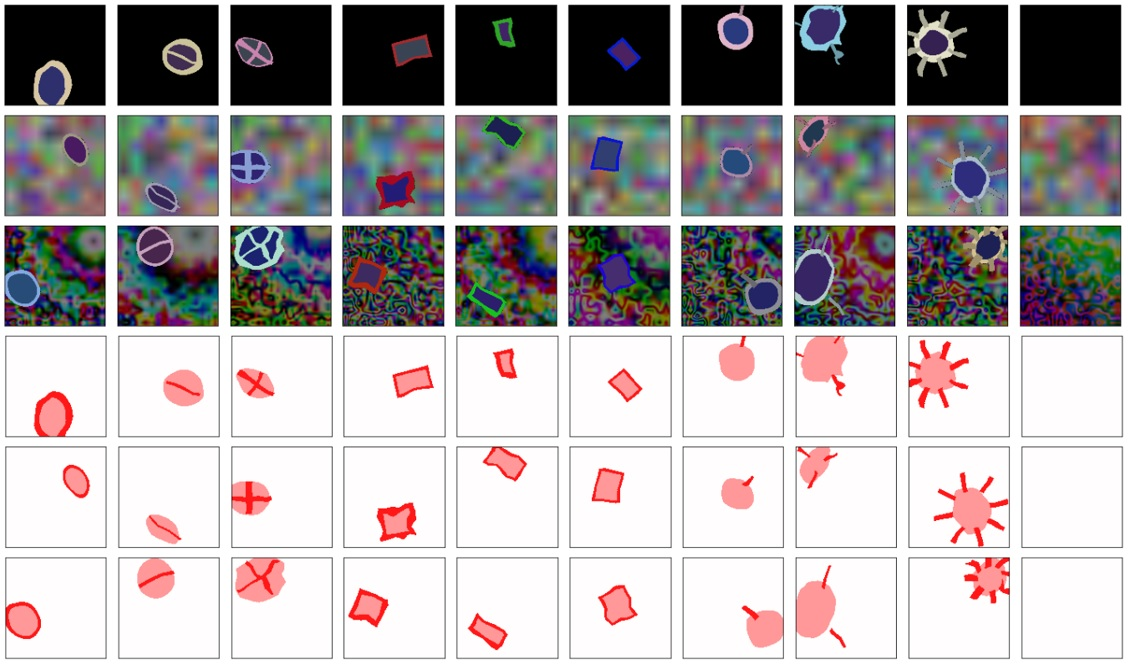
\includegraphics[width=1.0\textwidth]{fig_synthethic_paper_samples.jpeg}
    \caption[Synthetic dataset samples]{Synthetic dataset samples.}
    \caption*{Source: \href{https://github.com/ericotjo001/explainable\_ai}{https://github.com/ericotjo001/explainable\_ai}}
    \label{fig:synthetic_paper_samples}
    \end{center}
\end{figure}

Example data can be seen in Fig. \ref{fig:synthetic_paper_samples}. Ten different classes of cells are shown along the columns. Three types of backgrounds are given to increase the variation of dataset, as shown separately in the first three rows. The segmentation masks of the objects are shown in the bottom half of the figure. The classes are described in Table \ref{tab:synthetic_classes}.
\begin{table}[ht]
\centering
\begin{tabular}{rl}
  \toprule
  Class & Description \\
  \cmidrule(lr){1-2}
  0 & Circular cell with border\\
  1 & Circular cell with minus sign\\
  2 & Circular cell with plus sign\\
  3 & Rectangular cell in red\\
  4 & Rectangular cell in green\\
  5 & Rectangular cell in blue\\
  6 & Circular cell with one tail\\
  7 & Circular cell with three tails\\
  8 & Circular cell with eight tails\\
  9 & No cell\\
  \bottomrule
\end{tabular}
\caption[Synthetic dataset classes]{Synthetic dataset classes.}
\label{tab:synthetic_classes}
\end{table}

\subsubsection{Modifications to the baseline}
As the baseline dataset only contains single object instances, we changed the algorithms for generating images and annotations according to following criteria:
\begin{itemize}
    \item We omit class 9 as this class doesn't represent an object.
    \item We generate multiple datasets, each with a varying number of object instances and presence or absence of a background.
    \item Each dataset only has images with a fixed number of object instances. I.e., dataset 1 contains single-instance images, dataset 2 images only have 2 object instances, etc.
    \item All instances in an image are of the same class.
    \item For each image, we create bounding box and a segmentation mask annotations to evaluate localization performance.
    \item The segmentation masks cover the full object instance region. We don't make a distinction between edge and body of an object.
\end{itemize}
We extend the baseline dataset by generating datasets with multiple object instances in the synthetic images. In addition, bounding boxes and segmentation masks covering all object instances are created.

\subsubsection{Datasets}
According to the criteria in previous section, we have 8 different synthetic datasets as defined in Table \ref{tab:synthetic_datasets}.
\begin{table}[ht]
\centering
\begin{tabular}{lrll}
  \toprule
  Dataset & Instances & Background & Size\\
  \cmidrule(lr){1-4}
  synthetic\_d1b & 1 & yes & 512$\times$512\\
  synthetic\_d1t & 1 & no & 512$\times$512\\
  synthetic\_d2b & 2 & yes & 512$\times$512\\
  synthetic\_d2t & 2 & no & 512$\times$512\\
  synthetic\_d3b & 3 & yes & 512$\times$512\\
  synthetic\_d3t & 3 & no & 512$\times$512\\
  synthetic\_d4b & 4 & yes & 512$\times$512\\
  synthetic\_d4t & 4 & no & 512$\times$512\\
  \bottomrule
\end{tabular}
\caption[Synthetic datasets]{Synthetic datasets.}
\label{tab:synthetic_datasets}
\end{table}

Each dataset has a train, validation and test dataset of 1000, 200 and 200 images.

\subsection{ImageNet dataset}
Deng \textit{et al.} \cite{deng2009imagenet} introduced a database called "ImageNet”, a large scale ontology of images. It contains real, natural images with diverse objects covering 1000 distinct classes. We use the dataset that was used in the \acrfull{ilsvrc} competition for object localization. The dataset has images with multiple instances and ground-truth image-level labels and bounding boxes. It is a very popular dataset used in many papers.

We use the ImageNet dataset for the classification with localization tasks as defined for the \acrfull{ilsvrc} competition of 2012. The validation dataset consists of 50,000 photographs, collected from flickr and other search engines, hand labeled with the presence or absence of 1000 object categories and with bounding boxes. The training dataset is the subset of ImageNet containing the 1000 categories and 1.2 million images. The distribution of object instances over the images in the validation dataset is show in Fig. \ref{fig:imagenet_instance_distribution}.
\begin{figure}[ht]
    \begin{center}       
    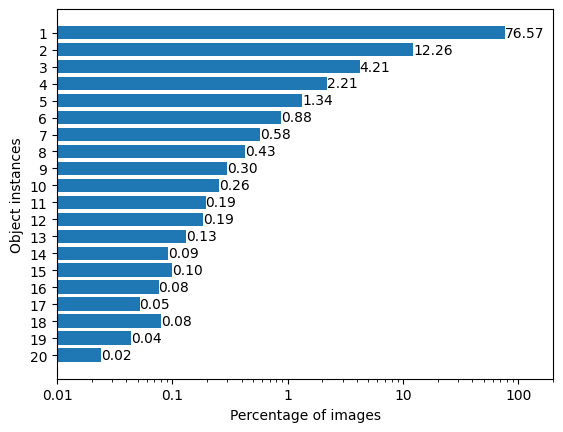
\includegraphics[width=0.7\textwidth]{fig_imagenet_distrib.png}
    \caption[ImageNet object instance distribution]{ImageNet object instance distribution.}
    \caption*{Source: Author}
    \label{fig:imagenet_instance_distribution}
    \end{center}
\end{figure}

\section{Training}
For the \acrlong{wsol} task, we only provide image-level labels to train a model for classification. At test time we will provide ground-truth bounding boxes and segmentation masks  to measure localization performance.

The \acrshort{cnn} is a feed-forward network. During the training process, the network will process the input through all the layers, compute the loss to understand how far the predicted label of the image is falling from the correct one, and propagate the gradients of network weights back into the network to update the weights of the layers. By iterating over a large dataset of inputs, the network will learn to set its weights to achieve the best results. The goal of training is to minimize the loss function. This optimization process requires iterating over the training data a number of times. One full iteration over the dataset is called an epoch.

\subsection{Data preprocessing}
Image preprocessing and image augmentations are two key processes taking place before images are fed to a neural network.

\subsubsection{Image preprocessing}
Image preprocessing are manipulations applied to images to create a common representations of different content. Following preprocessing operations are performed:
\begin{itemize}
    \item Resize: This operation resizes images to 256$\times$256 dimension for training and 224$\times$224 for inference.
    \item ToTensor: This operation converts an image's values in the range $[0, 255]$ to a tensor in the range $[0.0, 1.0]$.
\end{itemize}

\subsubsection{Data augmentation}
Image augmentation are manipulations applied to images to create different versions of similar content in order to expose the model to a wider array of training examples. For example, randomly altering rotation, brightness, or scale of an input image requires that a model consider what an image subject looks like in a variety of situations. Following augmentation operations are performed:
\begin{itemize}
    \item RandomCrop: Crops a given image at a random location to the size 224$\times$224.
    \item RandomHorizontalFlip: Horizontally flips a given image randomly with a given probability.
\end{itemize}

\subsection{Training process}
\subsubsection{Model initialization}
In order to build a model that accurately classifies images, the model weights must be initialized with proper values so that the model converges, i.e., minimizes the loss function.

We initialize weights of convolutional layers with values according to the method described by He \textit{et a.} \cite{he2015delving}, as this method is proven to provide good training results for \acrshort{cnn}s having \acrshort{relu} activation functions.

The weights of the fully-connected layers are initialized using random values from a normal distribution with standard deviation of 0.01. Using small initial weights avoids the vanishing and exploding gradients problem.

For training a model on the ImageNet dataset, we will use pre-trained model parameters as follows:
\begin{itemize}
    \item VGG16: Use pre-trained model for all \acrshort{cam} methods that don't require a network architecture with a \acrshort{gap} layer.
    \item VGG16-GAP: Parameters from layers common with the VGG16 model, are initialized with pre-trained parameters from the VGG16 model.
    \item ResNet-50: Use pre-trained model parameters for all \acrshort{cam} methods.
\end{itemize}

For training a model on the synthetic dataset, we will need to train the networks from scratch as this is a new dataset and thus no pre-trained network exists.

\subsubsection{Model training}
Supervised classification is an optimization problem where we want to minimize the loss, i.e. the difference between predicted and ground-truth class for the images in a dataset.

We use stochastic gradient descent for optimization of the loss function. We stop the learning process when the loss of the model on the validation dataset hasn't decreased for five subsequent training episodes.

\section{Localization} \label{lb:wsol_methods}
To localize object instances in images, we will benchmark a set of \acrshort{cam} related methods using models trained for classification on the synthetic and ImageNet datasets. The general process for localization is the same for all \acrshort{cam} methods. For each image of the validation or test dataset, following steps are performed:
\begin{enumerate}
    \item The neural network takes an image as input and returns a class prediction score.
    \item A score map is computed as a weighted combination of the feature maps in the final convolutional layer of the \acrshort{nn}. The weights are related to the ground-truth class of the image. The method to compute the weights is specific to the \acrshort{cam} method.
    \item The score map is normalized to values between 0 and 1.
    \item The normalized score map is binarized using a score map threshold. We use 100 different thresholds ranging from 0 to 1 with a step of 0.01, yielding 100 binarized score cams.
    \item For each binarized score map, we compute all self-contained contours. For those contours, bounding boxes are extracted. Bounding boxes are defined as a tuple with four coordinates ($(x_1, y_1, x_2, y_2)$ with $(x_1, y_1)$ the top-left coordinate and $(x_2, y_2)$ the bottom-right coordinate of the bounding box.
    \item For each score map, we keep track of the true positives and false positives, both for bounding boxes compared to ground-truth bounding boxes, and for binarized score maps compared to ground-truth segmentation masks.
    \item Localization accuracy is computed by counting predicted and ground truth label matches in the evaluation dataset
\end{enumerate}
When metrics are collected for all images, localization performance can be computed. The computation and evaluation of localization metrics are discussed in section \ref{sec:localization_metrics}. In the next sections we discuss the different \acrshort{cam}-based localization methods.

\subsection{CAM} \label{sec:cam}
Zhou \textit{et al.} proposes a general technique called \acrfull{cam} for \acrshort{cnn}s with \acrshort{gap} layer. A class activation map for a particular category indicates the discriminative image regions used by the
\acrshort{cnn} to identify that category. The procedure used for generating these maps is shown in Fig. \ref{fig:cam}. The \acrshort{gap} layer outputs the spatial average of the feature map of each channel of the last convolutional layer. The class-specific weights related to the \acrshort{gap} layer units, are then used to compute the weighted combination of the feature maps yielding the class activation map (or score map).

\begin{figure}[h]
    \begin{center}       
    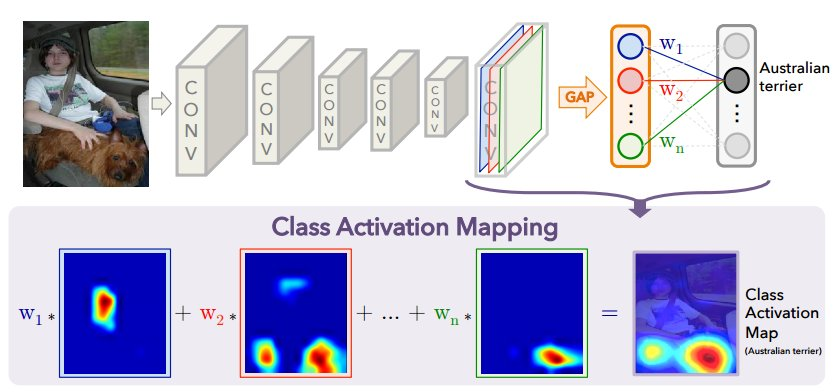
\includegraphics[width=1.0\textwidth]{fig_cam.jpeg}
    \caption[Class Activation Mapping]{Class Activation Mapping. The predicted class score is mapped back to the last convolutional layer to generate the class activation map. The \acrshort{cam} highlights the class-specific discriminative regions.}
    \caption*{Source: \href{https://github.com/zhoubolei/CAM}{https://github.com/zhoubolei/CAM}}
    \label{fig:cam}
    \end{center}
\end{figure}

We describe more formally how the \acrshort{cam} is computed. Let $f_{k}(x,y)$ be the activation of unit k in the final convolutional layer at spatial location $(x,y)$. Then, for unit k, the result of the \acrshort{gap} layer is:
\begin{equation} \label{eq:cam_gap}
    F^{k} = \sum_{x,y}f_{k}(x,y)
\end{equation}
For a given class c, the classification score $Y^{c}$ can be computed as:
\begin{equation} \label{eq:cam_score}
    Y^{c} = \sum_{k}w_{k}^{c}F_{k}
\end{equation}
Here, $w_{k}^{c}$ is the weight corresponding to class $c$ for unit $k$. It expresses the importance of $F_{k}$ for class $c$.
When we substitute equation \ref{eq:cam_gap} into \ref{eq:cam_score}, we get:
\begin{equation} \label{eq:cam_score2}
    Y^{c} = \sum_{k}w_{k}^{c}\sum_{x,y}f_{k}(x,y) = \sum_{x,y}\sum_{k}w_{k}^{c}f_{k}(x,y)
\end{equation}
Then the definition of the class activation map for class c for each spatial element is given by:
\begin{equation} \label{eq:cam_map}
    L_{CAM}^{c}(x,y) = \sum_{k}w_{k}^{c}f_{k}(x,y)
\end{equation}

The advantage of \acrlong{cam} is that it is able to localize discriminative image regions despite being trained for solving a classification task. In additon, it has low computational complexity as it needs only a single forward pass through the network to obtain the score map.

A disadvantage is, that the network only focuses on discriminative regions in an image, which leads to partial localization of objects. Another disadvantage of \acrshort{cam} is that it requires the network to have a \acrshort{gap} layer, which requires modifications in the network architecture. This change in an architecture causes a classification performance drop.

\subsection{Grad-CAM}
Selvaraju \textit{et al.} \cite{selvaraju2017grad} propose a technique called \acrfull{gradcam}. This approach uses the gradients of a class score, flowing into 
the final convolutional layer to produce a coarse localization map highlighting the important regions in the image for predicting the concept. 

\acrshort{gradcam} uses the final convolutional layer for localization as convolutional features retain spatial information that is lost in fully-connected layers and because the final convolutional layer can be expected to have the best compromise between high-level semantics and detailed spatial information. \acrshort{gradcam} uses the gradients of the neurons in the final convolutional layer to indicate the importance of each neuron for a predicted class.

\begin{figure}[ht]
    \begin{center}       
    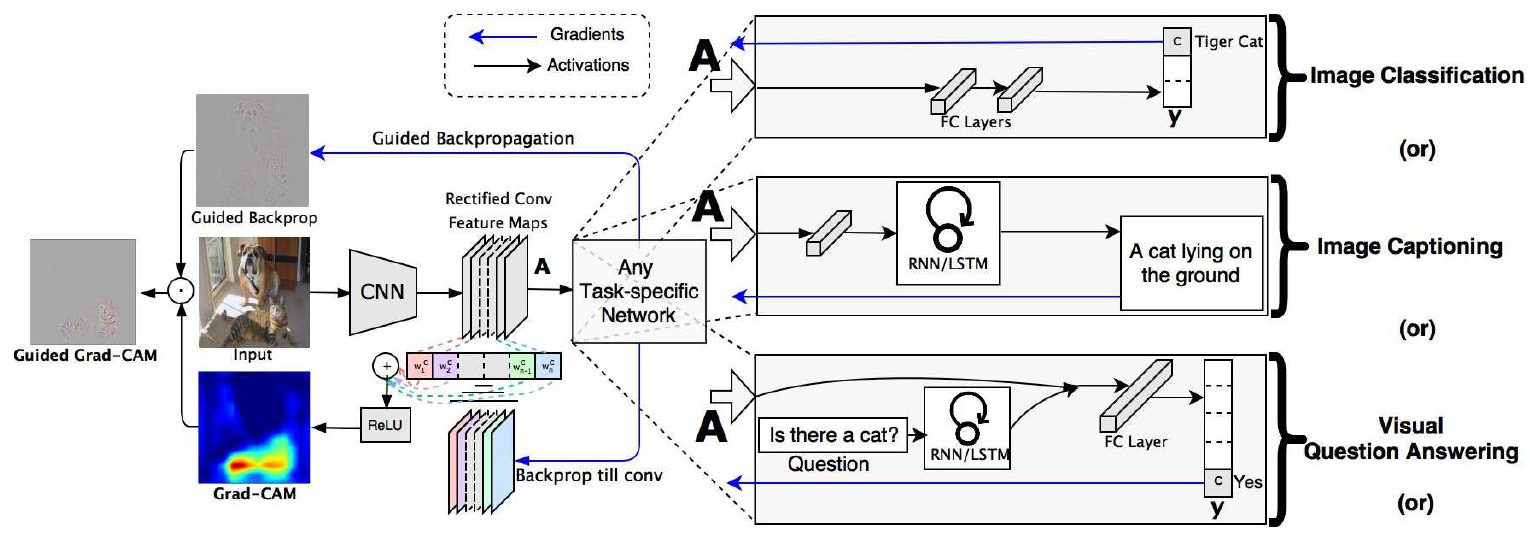
\includegraphics[width=1.0\textwidth]{fig_gradcam.png}
    \caption[Grad-CAM]{Grad-CAM. After forwarding an image through the network, a class score is obtained. The gradients of the desired class is then backpropagated to the feature maps of interest, which are combined using the average gradients per feature map as weights, yielding the \acrshort{gradcam} localization map.}
    \caption*{Source: Selvaraju \textit{et al.} \cite{selvaraju2017grad}}
    \label{fig:gradcam}
    \end{center}
\end{figure}
Fig. \ref{fig:gradcam} shows how the class-discriminative localization map is obtained. First the gradient of the score $Y^c$ for class $c$ is computed with respect to feature maps $A^k$ of a convolutional layer, i.e. $\frac{\partial{Y^c}}{\partial{A^k}}$. These gradients are then averaged to obtain the neuron importance weights $w_{k}^{c}$:
\begin{equation}
    w_{k}^{c} = \frac{1}{Z}\sum_{i}\sum_{j}\frac{\partial{Y^c}}{\partial{A_{ij}^{k}}}
\end{equation}

The weight $w_{k}^{c}$ captures the importance of a feature map $k$ for a target class $c$. The \acrshort{gradcam} localization map is then calculated as the weighted combination of feature maps, followed by a \acrshort{relu} activation function as we are only interested in features that have positive influence on the class of interest:
\begin{equation}
    L_{Grad-CAM}^{c} = ReLU \left( \sum_{k}w_{k}^{c} A^{k} \right)
\end{equation}

\acrshort{gradcam} is a generalization of \acrshort{cam}. It can be proven that when \acrshort{gradcam} is applied to architectures with a \acrshort{gap} layer, it specializes to the \acrshort{cam} method. Unlike the baseline \acrshort{cam} method, \acrshort{gradcam} is applicable to a wide variety of CNN model-families as it doesn't require an architecture with \acrshort{gap} layer.

\subsection{Grad-CAM++}
Chattopadhay \textit{et al.} \cite{chattopadhay2018grad} propose a technique called Grad-CAM++, to provide better localization of objects
as well as explaining occurrences of multiple objects of a class in a single image, compared with \acrshort{gradcam}. The proposed method uses a weighted combination of the positive partial derivatives of the last convolutional layer feature maps with respect to a specific class score as weights to generate a visual explanation for the class label under consideration. The Grad-CAM++ method, compared with CAM and Grad-CAM, is illustrated in Fig. \ref{fig:gradcamplusplus}.

\begin{figure}[h]
    \begin{center}       
    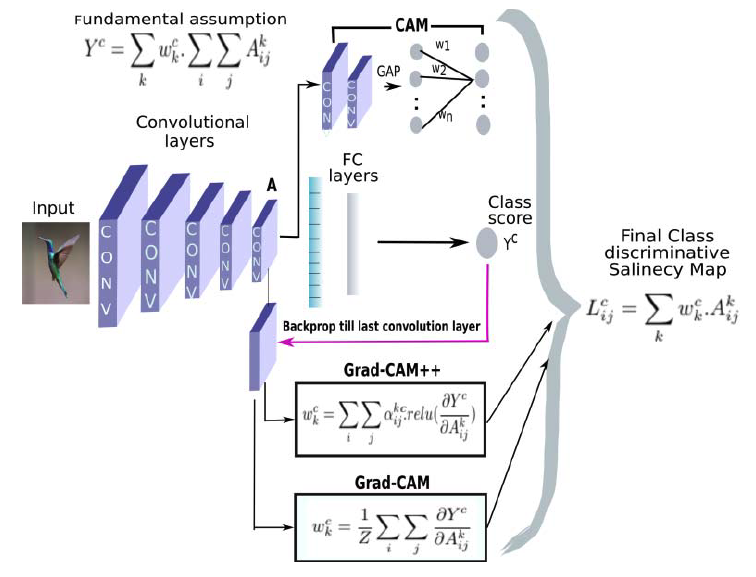
\includegraphics[width=1.0\textwidth]{fig_gradcamplusplus.png}
    \caption[Grad-CAM++]{Grad-CAM++, compared to Grad-CAM and CAM.}
    \caption*{Source: Chattopadhay \textit{et al.} \cite{chattopadhay2018grad}}
    \label{fig:gradcamplusplus}
    \end{center}
\end{figure}

The authors propose a more generalized method by explicitly coding the structure of the weights as:
\begin{equation}
    w_{k}^{c} = \sum_{i} \sum_{j} \alpha_{ij}^{kc} \dot ReLU \left( \frac{\partial{Y^c}}{\partial{A_{ij}^{k}}} \right)
\end{equation}
In this formulation, $w_{k}^{c}$ captures the importance of a particular activation map $A^k$. The weights are a weighted combination of the positive
partial derivatives with respect to each pixel in an activation map $A^k$ and capture the importance of that map for class $c$. Here, the weights $w_k^c$ are a weighted average of the gradients as opposed to a global average in Grad-CAM. $\alpha_{ij}^{k}$ is the weight of the gradient at spatial location $(x,y)$ in the feature map $A^k$. 

A formal derivation of the gradient weights is defined by Chattopadhay \textit{et al.} \cite{chattopadhay2018grad} and the result is given here for reference:
\begin{equation}
    \alpha_{ij}^{kc} = \frac{\frac{\partial^{2}{Y^c}}{\left( \partial{A_{ij}^{k}} \right)^2}}{2\frac{\partial^{2}{Y^c}}{\left( \partial{A_{ij}^{k}} \right)^2} + \sum_a \sum_b A_{ab}^{k} {\frac{\partial^{3}{Y^c}}{\left( \partial{A_{ij}^{k}} \right)^3}} }
\end{equation}
The time overhead for calculating higher order derivatives is of the same order as Grad-CAM as no cross higher-order derivatives are computed. The class-discriminative map for a given class $c$ is then computed as:
\begin{equation}
    L_{ij}^{c} = ReLU \left( \sum_{k}w_{k}^{c} A_{ij}^{k} \right)
\end{equation}

\subsection{Score-CAM}
Wang \textit{et al.} \cite{wang2020score} argue that gradient-based \acrshort{cam} methods can suffer from saturating gradients giving the false confidence that higher weights lead to high target scores. Score-CAM gets rid of the dependence on gradients by obtaining the weight of each activation map through its forward passing score on target class. The final score map is obtained by a linear combination of weights and activation maps.

In contrast to previous methods [4, 12], which use the gradient information flowing into the last convolutional layer to represent the importance of each activation map, Wang \textit{et al.} incorporate the importance as the Increase of Confidence: Given a function $Y = f(X)$ with input vector $X$ and output scalar $Y$, for a baseline input $X_b$, the contribution $c_i$ of $x_i$ towards $Y$ is the change of output by replacing the i-th entry in $X_b$ with $x_i$.
\begin{equation}
    c_i = f(X_b \odot H_i) - F(X_b)
\end{equation}
Where $H_i$ is a vector with the same shape of $X_b$ but for each entry $h_j$ in $H_i$, $h_i = \mathbb{I}[i=j]$ and $\odot$ denotes the Hadamard product.

Given a CNN model Y = f(X) that takes an input $X$ and outputs a scalar $Y$. We pick an internal convolutional layer $l$ in f and the corresponding activation as A. Denote the
k-th channel of $A_l$ by $A^k_l$ . For a known baseline input $X_b$,
the contribution $A^k_l$ towards $Y$ is defined as:
\begin{equation}
    C(A^k_l) = f(X o H^k_l) - f(X_b)
\end{equation}
where
\begin{equation}
    H^k_l = Normalize(Upsample(A^k_l))
\end{equation}
Finally, the score map is defined as:
\begin{equation}
    L^{c}_{Score-CAM} = ReLU(\sum_{k} \alpha^{c}_{k} A^k_l)
\end{equation}
where
\begin{equation}
    \alpha^{c}_{k} = C(A^k_l)
\end{equation}
Fig. \ref{fig:scorecam} shows the pipeline for Score-CAM. Activation maps are first extracted in Phase 1. For each activation map then, the original image is masked with the original image in phase 2 and fed to the network again. The obtains score on the target class is then used as the weight of the activation maps. Finally, the score map is generated by the weighted combination of activation maps. Phase 1 and Phase 2 share the same CNN module as feature extractor. 
\begin{figure}[h]
    \begin{center}       
    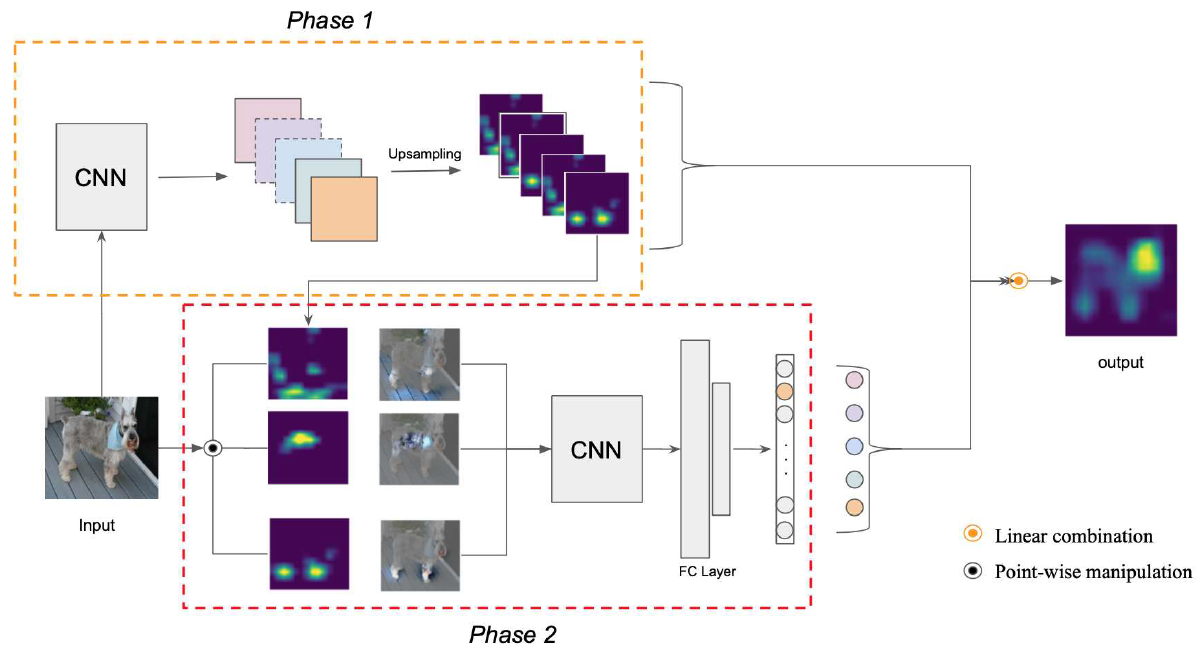
\includegraphics[width=1.0\textwidth]{fig_scorecam.png}
    \caption[Score-CAM]{Score-CAM.}
    \caption*{Source: Wang \textit{et al.} \cite{wang2020score}}
    \label{fig:scorecam}
    \end{center}
\end{figure}

Score-CAM shows more focus on object instances and is also promising for capturing the features of multiple instances in the explanation map. A major disadvantage of Score-CAM is the computational cost because it requires as many as feature maps in the last convolutional layer more forward passes than the baseline \acrshort{cam} method.

\subsection{MinMaxCAM}
One of the most common problems of methods based on Class Activation Mapping,
is caused either by localization maps which focus, exclusively, on the most discriminative region of the objects of interest, or by activations occurring
in background regions. To address these two problems, Wang \textit{et al.} \cite{wang2021minmaxcam} propose two representation regularization mechanisms: Full Region Regularization which tries to maximize the coverage of the localization map inside the object region, and Common Region Regularization which minimizes the activations occurring in background regions.

The idea of the Common region regularization (CRR) is that different images depicting foreground objects of the same class should share similar features. The localized-object features can be obtained by applying the normalized Class Activation Map (CAM) $H$ (extracted as is done for the CAM method in section \ref{sec:cam}) on the image $I$ and extract the feature of $I \odot H$, denoted as $f$. Therefore, $f = B(I \odot H)$, where $\odot$ refers to the element-wise multiplication. To save computational resources, we use the same backbone B both for CAM computation and regularization. Given S different images from the same class, we have:
\begin{equation}
    CRR = \frac{1}{S(S-1)} \sum^{S-1}_{i=0} \sum^{S-1}_{j=0} \lVert f_i - f_j \rVert^2_2
\end{equation}
CRR calculates the pair-wise distance of the feature of $IoH$. The goal of CRR is to localize the common region of a set of images from the same class. By minimizing it, it can minimize the activations on the localization map, i.e. suppress the activations in non-object regions of the images.

For the case of the failed localization on the most discriminative region, the authors propose Full region regularization (FRR) to enlarge the localization map.

\begin{equation}
    FRR = \frac{1}{S} \sum^{S-1}_{i=0}\lVert f_i - f^o_i \rVert^2_2
\end{equation}
$f^o$ is the feature of the original image $I$, i.e. $f^o=B(I)$. FRR calculates the distance of the feature between the $IoH$ and $I$. Minimizing FRR has the effect of maximizing the activations on the localization map.

The learning process has two stages. For stage I, it takes $N x S$ images as input. The model is trained for the classification task, i.e. update the backbone and linear layer via the cross-entropy loss. It is the same as CAM.

For stage II, the backbone B is frozen as a feature extractor. It receives the images multiplied by the localization map $(I \odot H)$ as input.

The features ($f$ and $f^o$) extracted by B are used for the two regularizations. The loss only updates the weights of the linear layer, by minimizing CRR and FRR:
\begin{equation}
    L_{S2} = \lambda_{1}CRR + \lambda_{2}FRR
\end{equation} 
LS1 and LS2 update the model every mini-batch. Fig. \ref{fig:minmaxcam} shows the proposed method.
\begin{figure}[ht]
    \begin{center}       
    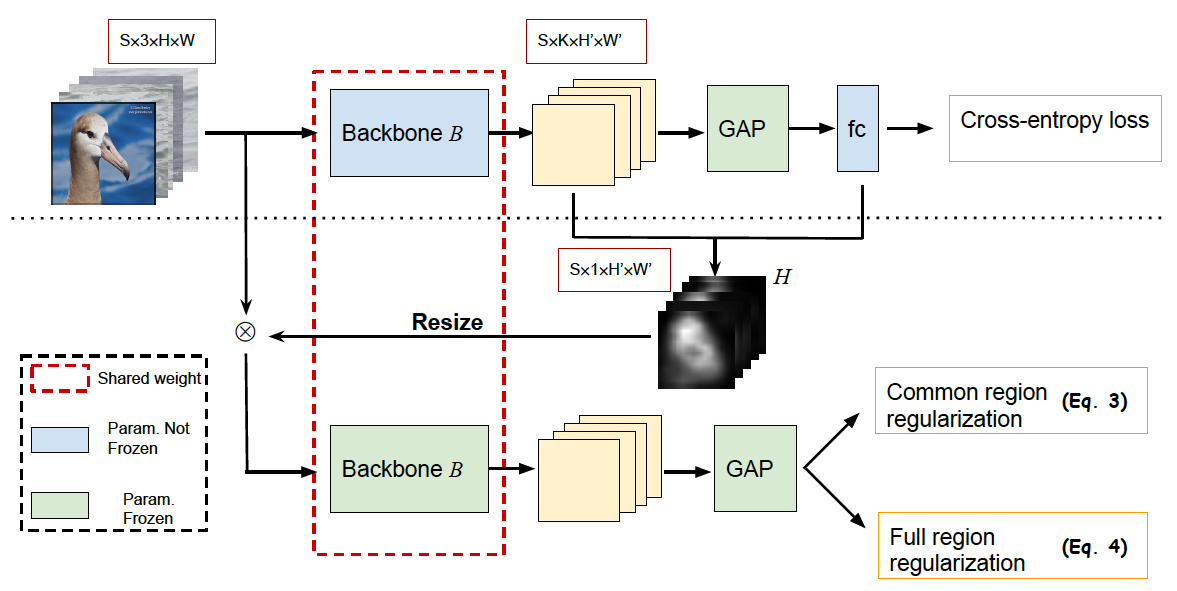
\includegraphics[width=1.0\textwidth]{fig_minmaxcam.png}
    \caption[MinMaxCAM]{MinMaxCAM.}
    \caption*{Source: Wang \textit{et al.} \cite{wang2021minmaxcam}}
    \label{fig:minmaxcam}
    \end{center}
\end{figure}

\section{Evaluation}
\subsection{Computational complexity} \label{sec:computational_complexity}
An important aspect of any algorithm is its computational complexity, i.e., a measure of the amount of computing resources (time and space) that a particular algorithm consumes when it runs. While the initial focus in research may be on maximizing accuracy of an algorithm, it is also important to focus on maximizing the inference efficiency. The efficiency of an algorithm may determine whether it is a viable solution. In this section we specify the metrics we use to measure the algorithm complexity in our experiments. From a theoretical perspective, we reason about the complexity of the different \acrshort{cam} methods used for localization.

\subsubsection{Complexity metric}
Geifman \cite{article:FLOPSvsRuntime} reasons that it is wrong to assume that \acrfull{flop} can serve as an accurate proxy for any kind of efficiency, including run-time. Due to high parallelization capabilities of the \acrshort{gpu}, parallelizable operations will run faster. Moreover, some operations may require the same number of \acrshort{flop}s, but different run time, depending on how well the operations can be accelerated on a \acrshort{gpu}. Another problem is that many \acrshort{flop} count tools only measure forward passes in a model. This is not sufficient for gradient-based \acrshort{cam} methods which require backward passes through the model to compute gradients.

This is why we measure the run time of \acrshort{cam} methods. Given equal hardware and parallelization capabilities, a fair comparison can be made between algorithms. To correctly measure the run time of the \acrshort{cam} methods we take into account following aspects:
\begin{enumerate}
    \item We don't measure \acrshort{gpu} warm-up time, i.e. the time a \acrshort{gpu} device needs to go from low-power state to operational state. We don't measure that time, because it is not relevant for the comparison of the methods. Before measuring starts, we send random data through a dummy model to force the \acrshort{gpu} in its operational state.
    \item Data loading, pre-processing and transferring between \acrshort{cpu} and \acrshort{gpu} is not measured.
    \item  Time recording takes place only after the process running on the \acrshort{gpu} is finished, i.e., when \acrshort{gpu} and \acrshort{cpu} are synchronized.
\end{enumerate}
\subsubsection{Comparison from theoretical perspective}
Based on the design of the \acrshort{cam} methods, we can theoretically reason about their computational complexity. Table \ref{tab:complexity_theoretical} shows a comparison.
\begin{table}[ht]
\centering
\begin{tabular}{lcc}
  \toprule
  method & forward passes & backward passes\\
  \cmidrule(lr){1-3}
  \addlinespace[0.5em]
  CAM & $\begin{aligned} \frac{N}{B} \end{aligned}$ & $\begin{aligned}0\end{aligned}$\\
  \addlinespace[0.5em]
  Grad-CAM   & $\begin{aligned} \frac{N}{B} \end{aligned}$ & $\begin{aligned} \frac{N}{B}\end{aligned}$\\
  \addlinespace[0.5em]
  Grad-CAM++ & $\begin{aligned} \frac{N}{B} \end{aligned}$ & $\begin{aligned} \frac{N}{B}\end{aligned}$\\
  \addlinespace[0.5em]
  MinMaxCAM & $\begin{aligned} \frac{N}{B} \end{aligned}$ & $\begin{aligned}0\end{aligned}$\\
  \addlinespace[0.5em]
  Score-CAM &  $\begin{aligned} \frac{N}{B} + N \times \frac{F}{B_F} \end{aligned}$ & $\begin{aligned}0\end{aligned}$\\
  \addlinespace[0.5em]
  \bottomrule 
\end{tabular}
\caption[Theoretical complexity of CAM methods]{Theoretical complexity of CAM methods. $N$: number of images in dataset, $B$: image batch size, $F$: number of feature maps in last \acrshort{cnn} layer, $B_F$: feature map batch size.}
\label{tab:complexity_theoretical}
\end{table}

MinMaxCAM uses CAM as localization method, so it has the same inference time. MinMaxCAM has longer training time due to its regularization, but this is not taken into account for the localization task itself. Both CAM and MinMaxCAM have the lowest computational cost as they only require a single forward pass per batch of images. Grad-CAM and Grad-CAM++ are gradient-based methods and need an additional backward pass through the network to compute the gradients. If we take the assumption that forward pass and backward pass have the same order of complexity, then Grad-CAM and Grad-CAM++ have roughly double the run time of CAM. Score-CAM requires many forward passes: It gets the features maps, as the other methods do. For those feature maps, it then needs a forward pass of the original images ablated with the feature maps to get the weights computed as confidence scores. It does so in batches. This explains the $\begin{aligned}N\frac{F}{B_F}\end{aligned}$ term in the number of forward passes. Score-CAM requires $F + 1$ times more forward passes than CAM in case the image batch size $B$ and feature map batch size $B_F$ are equal. For a ResNet-50 network with 2048 feature maps in the final convolutional layer, this is a costly operation.

\subsection{Localization metrics} \label{sec:localization_metrics}
To objectively evaluate and compare object localization using different \acrshort{cam} methods, we need to quantitatively determine performance using localization metrics. The papers introducing the \acrshort{cam} methods, specify different metrics: Zhou \textit{et al.} \cite{zhou2016cvpr} (\acrshort{cam}) and Selvaraju \textit{et al.} \cite{selvaraju2017grad} (\acrshort{gradcam}) use the localization error, which is defined for localization of a single object instance. Chattopadhay \textit{et al.} \cite{chattopadhay2018grad} (\acrshort{gradcam}++) evaluate localization using faithfulness based metrics. These metrics measure drop or increase of prediction scores, rather than localization of object instances. Wang \textit{et al.} \cite{wang2020score} evaluates localization from an energy-based perspective at pixel-level. None of the mentioned methods is thus usable for measuring localization performance of multiple object instances.

We set out following criteria for choosing localization metrics:
\begin{enumerate}
    \item The metrics must be applicable to all evaluated \acrshort{cam} methods
    \item Metrics must be applicable for datasets with bounding boxes ground-truth and for datasets with segmentation mask ground-truth
    \item Localization accuracy of multiple object instances is measured
\end{enumerate}

Choe \textit{et al.} \cite{choe2020evaluating} have defined a \acrshort{wsol} evaluation protocol, defining metrics that are applicable to all evaluated \acrshort{cam} methods, meeting criterion 1. The authors defined a metric that measures maximum box accuracy for datasets with ground-truth bounding boxes, and a metric that measures pixel average precision for datasets with ground-truth segmentation masks. This covers criterion 2. However, criterion 3 is not met, as the maximum box accuracy doesn't take into account measuring of multiple instances.

We enhance the evaluation metrics of Choe \textit{et al.} to measure localization of multiple object instances for the \acrshort{wsol} task, thereby meeting criterion 3.

\subsubsection{Recall versus precision}
We could have a localization method that exhaustively generates bounding boxes of different granularity. In that case, the localization method will have a high recall: It will accurately localize most object instances. At the same time that method will suffer from a lot of false positives, i.e., many localized objects would not match with the actual ground truth instances. 

Ideally, we would like to have a localization method that has good precision and recall. If we equally care about precision and recall, the f1 score represents the harmonic mean between precision and recall. 

Here we illustrate how precision, recall and f1 score are determined in the experiments for localization. To compute precision and recall, we need to define the confusion matrix for the localization task. 

A confusion matrix is made up of 4 components, namely, \acrfull{tp}, \acrfull{tn}, \acrfull{fp} and \acrfull{fn}. To define all the components, we need to define some \acrshort{iou} threshold. If the overlap between an estimated and ground truth bounding box is at least the \acrshort{iou} threshold, we have a match and the object instance is said to be localized. The parameters of a confusion matrix are shown in Table \ref{tab:confusion_matrix}.
\begin{table}[ht]
\centering
\begin{tabular}{l|l|c|c|}
\multicolumn{2}{c}{} & \multicolumn{2}{c}{Ground truth} \\
\cline{3-4}
\multicolumn{2}{c|}{} & positive & negative \\
\cline{2-4}
\multirow{2}{*}{Predicted} & positive & TP & FP \\
\cline{2-4}
                           & negative & FN & TN \\
\cline{2-4}
\end{tabular}
\caption[Confusion matrix]{Confusion matrix.}
\label{tab:confusion_matrix}
\end{table}

Both for ground truth and predicted bounding boxes, there are two cases: There is a bounding box (positive) or there isn't one (negative). The confusion matrix parameters are then defined as follows
\begin{itemize}
    \item \textbf{TP}: A predicted bounding box that matches with a ground truth bounding box, i.e., their intersection over union is at least the \acrshort{iou} threshold.
    \item \textbf{FP}: A predicted bounding box that overlaps less than the \acrshort{iou} threshold with the ground truth bounding boxes.
    \item \textbf{FN}: A false negative is a ground truth object that is not localized. 
    \item \textbf{TN}: A true negative is every part of the image for which we don't have a ground truth bounding box, and where we did not predict an object. This metric is not useful for object localization, hence we ignore it by setting it to zero.
\end{itemize}
Now that we know what the parameters represent, we can formally define the equations for these parameters, as shown in Table \ref{tab:confusion_matrix_definitions}.
\begin{table}[ht]
\centering
\begin{tabular}{lll}
  \toprule
  Metric & & Remark\\
  \cmidrule(lr){1-1} \cmidrule(lr){3-3}
  $TP$ & & Number of matching predicted boxes and ground truth boxes\\
  $\begin{aligned} FP = P - TP \end{aligned}$ & & $P$: Number of predicted boxes\\
  $\begin{aligned} FN = G - TP \end{aligned}$ & &$G$: Number of ground truth boxes \\
  $\begin{aligned} TN = 0 \end{aligned}$ & & Not relevant for localization task\\
  \bottomrule 
\end{tabular}
\caption[Confusion matrix definitions]{Confusion matrix definitions}
\label{tab:confusion_matrix_definitions}
\end{table}

Recall can be defined as the proportion of ground truth objects $G$ that are correctly detected:
\begin{equation} \label{eq:recall}
Recall = \frac{TP}{TP + FN} = \frac{TP}{G}
\end{equation}

Precision can be thought of as the proportion of all detected object instances $P$ that are correct:
\begin{equation} \label{eq:precision}
Precision = \frac{TP}{TP + FP} = \frac{TP}{P}
\end{equation}

The f1 score can then be computed:
\begin{equation} \label{eq:f1}
F1 = 2 \times \frac{Precision \times Recall}{Precision + Recall}
\end{equation}

%- What if an image has 1 large object instance and 1 small instance?
%- Is the metrics only saying something about the large instance?
%- What is the intended use of the metrics?
%- Do you want to find all instance in an image or are you using a metric that is good at measuring localization but not good at finding all instances?
\subsubsection{MaxBoxAccV3 metric} \label{sec:method_maxboxaccv3}
Many datasets only provide bounding box annotations, as segmentation masks are expensive to collect. This is the case for the ImageNet dataset. For this case, we define a metric that measures how accurate ground truth bounding box annotations match with bounding boxes extracted by the \acrshort{cam} localization methods.

Here, we derive the multi-instance localization metric $MaxBoxAccV3$ step by step, starting with metrics defined by Choe \textit{et al.} \cite{choe2020evaluating}.

Given a dataset with N images and ground truth boxes B, the box accuracy at score map threshold $\tau$ and a \acrshort{iou} threshold $\delta$ is defined as:
\begin{equation} \label{eq:boxacc}
    BoxAcc(\tau,\delta) := \frac{1}{N} \sum_{n=1}1_{IoU(box(s(X^{(n)}),\tau),B^{(n)})\ge\delta}
\end{equation}
where $box(s(X^{(n)}))$ is the tightest bounding box around the largest-area connected component in the score map \{$(i,j)\text{ }|\text{ }s(X^{(n)}_{ij}) \ge \tau$\}. The amount of overlapping between the predicted bounding box and ground truth bounding box expresses how accurate the localization method is. The overlapping is computed as the proportion of area of the boxes that overlap versus the total area of both boxes. The \acrfull{iou} metric captures this overlap and is illustrated in Fig. \ref{fig:iou}. This metric is also used frequently in object detection challenges such as the Pascal VOC challenge \cite{everingham2009pascal}. The \acrshort{iou} produces a number between $0$ and $1$. The closer \acrshort{iou} is to 1, the better the localization is. We will use an \acrshort{iou} threshold $\tau$ to assess whether the amount of overlap is sufficient to consider the localization a true positive match.
\begin{figure}[ht]
    \begin{center}       
    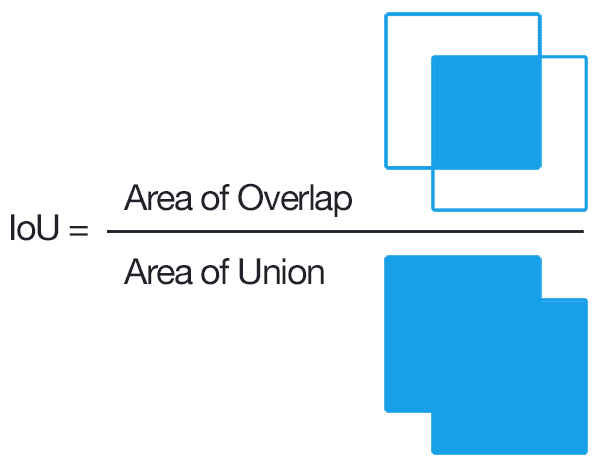
\includegraphics[width=0.3\textwidth]{fig_iou.png}
    \caption[The IoU equation]{The Intersection over Union equation.}
    \caption*{Source: href{https://pyimagesearch.com/2016/11/07/intersection-over-union-iou-for-object-detection}{https://pyimagesearch.com/2016/11/07/intersection-over-union-iou-for-object-detection}}
    \label{fig:iou}
    \end{center}
\end{figure}

We then count the number of images where the predicted bounding box overlaps with ground truth box $B$ with $IoU \ge \delta$, and average the count over the number of images. This gives a box accuracy score between $0$ and $1$. For datasets with images where more than one ground truth bounding box is provided, e.g. ImageNet, we count the number of images where box prediction overlaps with at least one of the ground truth bounding boxes with $IoU \ge \delta$. When $\tau$ is 0.5, the metric is commonly-called GT-known localization accuracy. 

For score map threshold independence, the box accuracy is reported at the optimal threshold $\tau$, i.e., the \textbf{maximal box accuracy}:
\begin{equation}
    MaxBoxAcc(\tau) := max_{\tau} BoxAcc(\tau,\delta)
\end{equation}

Choe \textit{et al.} \cite{choe2020evaluating} sets $\delta = 0.5$ for $MaxBoxAcc$ to follow prior works. The authors developed an improved version called $MaxBoxAccV2$ that is better for two reasons: $MaxBoxAcc$ measures performance at fixed \acrshort{iou} threshold ($\delta = 0.5$). $MaxBoxAccV2$ averages performance across $\delta \in$ {0.3, 0.5, 0.7} to account for different levels of localization fineness. $MaxBoxAcc$ takes the largest connected component in the score map for estimating the bounding box, assuming that the object of interest will be large. This assumption is dropped by $MaxBoxAccV2$, which considers the best match between the set of detected bounding boxes and ground truth bounding boxes. Choe \textit{et al.} encourage to use $MaxBoxAccV2$ for future \acrshort{wsol} research. $MaxBoxAccV2$ is thus defined as:
\begin{equation} \label{eq:maxboxaccv2}
    MaxBoxAccV2(\tau) := \frac{1}{3} \sum_{\delta \in (0.3,0.5,0.7)} max_{\tau} BoxAcc(\tau,\delta)
\end{equation}

As $MaxBoxAccV2$ considers the best match between the set of estimated and ground truth bounding boxes, it is not suited for measuring multiple-instance localization performance. We will enhance $MaxBoxAccV2$ to account for multiple instances. To this purpose, the definition of box accuracy must be revised to $BoxAccV2$:
\begin{equation} \label{eq:boxaccv2}
    BoxAccV2(\tau,\delta) := \frac{1}{G} \sum^{N}_{n=1} \sum^{G^{(n)}}_{g=1}  1_{IoU(box(s(X^{(n)}),\tau),B^{(n)})\ge\delta}
\end{equation}

The n-th image in dataset $X$ is denoted as $X^{(n)}$. The \acrshort{cam} method produces the score map $s(X^{(n)})$ and estimated set of bounding boxes $box(s(X^{(n)}),\tau)$ at score map threshold $\tau$. The set of ground truth bounding boxes for image n is $B^{(n)}$. The number of images in the dataset is $N$, the number of ground truth boxes in image n is $G^{(n)}$ and the total number of ground truth boxes in the dataset is $G$. The major difference with Equation \ref{eq:boxacc} is that in Equation \ref{eq:boxaccv2} we have an additional inner iteration where for each ground truth bounding box in an image, we try to find a match with the set of estimated bounding boxes for that image. In this inner iteration, there can only be a single match between a ground truth box and an estimated box at any time.

We then define $MaxBoxAccV3$ as:
\begin{equation} \label{eq:maxboxaccv3}
    MaxBoxAccV3(\tau) := \frac{1}{3} \sum_{\delta \in (0.3,0.5,0.7)} max_{\tau} BoxAccV2(\tau,\delta)
\end{equation}
With this definition we meet the third criterion for a metric that measures multiple-instance localization performance.

$BoxAccV2$ in equation \ref{eq:boxaccv2} has in its numerator the total number of matching ground truth and predicted bounding boxes. These are the true positives, as defined in Table \ref{tab:confusion_matrix_definitions}. The denominator is the number of ground truth bounding boxes. Taking into account the definition for recall in Equation \ref{eq:recall}, we can formulate $BoxAccV2(\tau, \delta)$ as the recall at score map threshold $\tau$ and IoU threshold $\delta$. Hence, $MaxBoxAccV3$ in Equation \ref{eq:maxboxaccv3} then represents the average recall for $IoU \in (0.3, 0.5, 0.7)$ at the optimal score map threshold $\tau$.

\subsubsection{PxAP metric}
When ground truth masks are available for evaluation, pixel-wise precision and recall can be measured. These metrics allow users to choose the preferred operating score map threshold $\tau$ that provides a trade-off between precision and recall. Choe \textit{et al.} define the \textbf{pixel-wise precision and recall at threshold $\tau$} as:
\begin{equation} \label{eq:pxprec}
    PxPrec(\tau) = \frac{\lvert \{ s^{(n)}_{ij} \ge \tau \} \cap \{ T^{(n)}_{ij} = 1 \} \rvert}{\lvert \{ s^{(n)}_{ij} \ge \tau \} \rvert}
\end{equation}
and:
\begin{equation} \label{eq:pxrec}
    PxRec(\tau) = \frac{\lvert \{ s^{(n)}_{ij} \ge \tau \} \cap \{ T^{(n)}_{ij} = 1 \} \rvert}{\lvert \{ T^{(n)}_{ij} = 1 \} \rvert}
\end{equation}

Pixel-wise precision in Equation \ref{eq:pxprec} computes the proportion of the pixels in the score map $\{ s^{(n)}_{ij} \ge \tau \}$ that match the foreground pixels of the ground truth mask $\{ T^{(n)}_{ij} = 1 \}$. Pixel-wise recall indicates the proportion of the number of foreground pixels in the ground truth mask that are matched by the pixels in the score map at threshold $\tau$. For threshold independence, the \textbf{pixel average precision} is defined:
\begin{equation}
    PxAP := \sum_{l} PxPrec(\tau_{l})(PxRec(\tau_{l}) - PxRec(\tau_{l-1}))
\end{equation}
This metric is the area under the curve of the pixel precision-recall curve. As the metric measure localization at pixel level, it can be used to evaluate multiple-instance localization, and therefore the third localization criterion is met.

\section{Localization improvement} \label{sec:method_localization_improvement}
A challenge of using a single operational threshold for masking the score map and during localization, is that not all object instances in an image may be of similar intensity. An intuition is that as the \acrshort{wsol} task is trained for classification, it will activate on the most discriminative parts of the image that are related to the targeted class. Some object instances may  have more outspoken features that activate during inference. For classification to be accurate, it's not necessary for the network to activate equally strong on all object instances.

Based on the formulated intuition, we propose an iterative localization method where we mask previously found object instance locations in the original image and apply the localization method again to find additional object instance locations. The process is as follows:

\begin{enumerate}
    \item In the first iteration, all images of the test dataset are fed to the \acrshort{cam} localization method. Bounding boxes are computed for various score map thresholds. From all these thresholds and bounding boxes, the $MaxBoxAccV3$ metric is computed yielding the optimal score map threshold. The bounding boxes estimated at the optimal threshold are saved.
    \item In a next iteration, all images of the dataset are masked with bounding boxes extracted during the previous iteration. We test different mask strategies: Mask with zero values, mean image value, random values drawn from the image dataset distribution. The masked images are fed to the \acrshort{cam} localization method to extract bounding boxes and compute the $MaxBoxAccV3$ metric. Newly found bounding boxes are added to boxes found during previous iterations according to a bounding box merge strategy: 'Add' unconditionally adds boxes to the list of boxes from previous iterations. If boxes overlap more than 20\%, 'Drop' removes boxes and 'Merge' unifies the boxes by calculating the box surrounding both boxes. If a box overlaps less than 20\% with an existing box, it is added to the list of boxes. Masked images that cause a drop in classification score that exceeds a predefined threshold, will stop contributing to this iterative process of finding additional object instances. This predefined drop threshold is a parameter that can be tuned.
    \item The second step is repeated until a predefined number of iterations  has executed.
\end{enumerate}

\section{Implementation references}
We based our evaluation method on existing implementations and extended them to implement \acrlong{mwsol}. The software implementations we enhanced is listed here for reference:
\begin{itemize}
    \item CAM \cite{code:CAM}: The baseline CAM method.
    \item MinMaxCAM \cite{code:MinMaxCAM}: The MinMaxCAM training algorithm.
    \item WSOLevaluation\cite{code:WSOLevaluation}: The single-instance \acrshort{wsol} evaluation metrics.
    \item PytorchCAM \cite{code:PytorchCAM}: Inference methods for Grad-CAM, Grad-CAM++ and Score-CAM.
\end{itemize}